\documentclass[11pt, letterpaper]{article}
\input{../../../../report.tex}
\usepackage{titlepageBU}
\title{Excursion 1}
\date{10/07/24}
\courseID{MA 291}
\professor{Dr. Borkovitz}
\courseSection{A1}
\renewcommand{\mod}[1]{\;(\text{mod}\;#1)}
\hypersetup{
	colorlinks=true,
	linkcolor=blue,
	urlcolor=blue,
	citecolor=blue,
}
\contributor{Emir}
\contributor{Max W.}
\contributor{Nathan}
\contributor{Edison}
\usepackage{pgfplots}
\pgfplotsset{width=17cm,compat=1.18}
\definecolor{fgreen}{RGB}{0, 150, 0}
\begin{document}
\begin{center}
	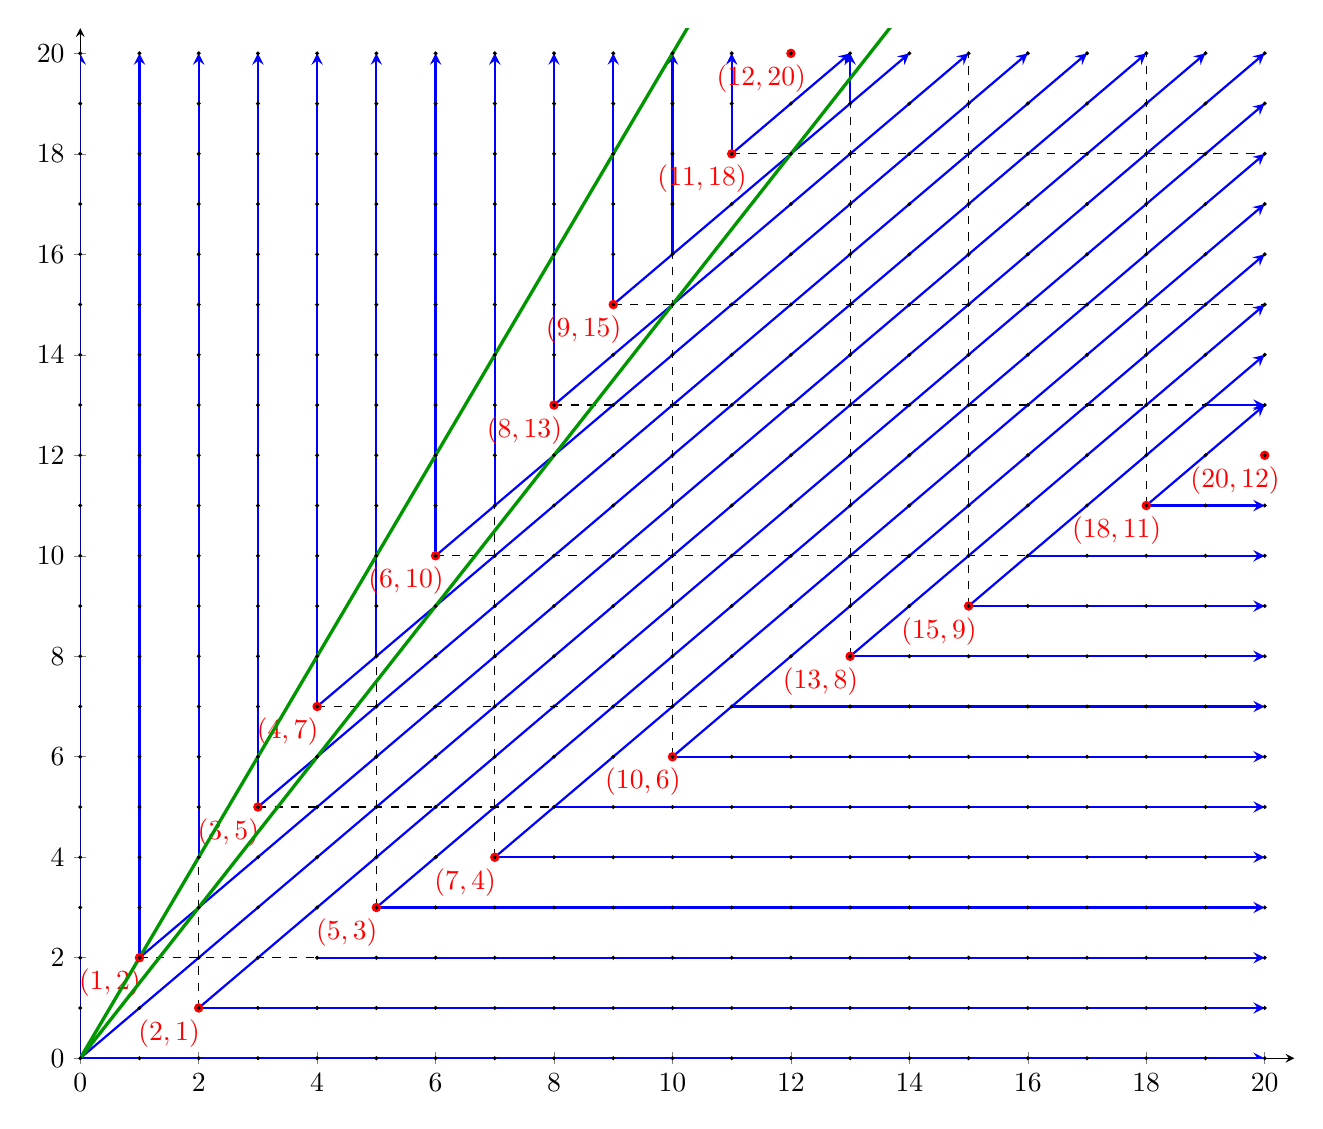
\begin{tikzpicture}
		\begin{axis}[
				xmin=0, xmax=20.5,
				ymin=0, ymax=20.5,
				axis lines = left,
			]
			\addplot[blue, thick, quiver={u=\thisrow{u},v=\thisrow{v}},-stealth] table {
				x y u v
				0 0 0 20
				0 0 20 0
				0 0 20 20
				2 1 18 0
				2 1 18 18
				2 4 0 16
				1 2 0 18
				1 2 18 18
				4 2 16 0
				3 5 0 15
				3 5 15 15
				8 5 12 0
				5 3 15 0
				5 3 15 15
				5 8 0 12
				4 7 0 13
				4 7 13 13
				11 7 9 0
				7 4 13 0
				7 4 13 13
				7 11 0 9
				6 10 0 10
				6 10 10 10
				16 10 4 0
				10 6 10 0
				10 6 10 10
				10 16 0 4
				8 13 0 7
				8 13 7 7
				19 13 1 0
				13 8 7 0
				13 8 7 7
				13 19 0 1
				9 15 0 5
				9 15 5 5
				15 9 5 0
				15 9 5 5
				11 18 0 2
				11 18 2 2
				18 11 2 0
				18 11 2 2
			};
		\addplot[black, dashed, quiver={u=\thisrow{u},v=\thisrow{v}}] table {
				x y u v
				2 1 0 3
				1 2 3 0
				3 5 5 0
				5 3 0 5
				7 4 0 7
				4 7 7 0
				6 10 10 0
				10 6 0 10
				8 13 11 0
				13 8 0 11
				9 15 11 0
				15 9 0 11
				11 18 9 0
				18 11 0 9
			};
		\addplot[red, only marks, mark=*, mark size=1.5pt] coordinates {
				(2,1)(1,2)(3,5)(5,3)(4,7)(7,4)(6,10)(10,6)(8,13)(13,8)(9,15)(15,9)(11,18)(18,11)(12,20)(20,12)
			};
			\foreach \x in {0,...,20} {
				\foreach \y in {0,...,20} {
					\addplot[black, only marks, mark=*, mark size = 0.5] coordinates {(\x,\y)};
				};
			};
			\draw node[red] at (0.5,1.5) {$(1,2)$};
			\draw node[red] at (2.5,4.5) {$(3,5)$};
			\draw node[red] at (3.5,6.5) {$(4,7)$};
			\draw node[red] at (5.5,9.5) {$(6,10)$};
			\draw node[red] at (7.5,12.5) {$(8,13)$};
			\draw node[red] at (8.5,14.5) {$(9,15)$};
			\draw node[red] at (10.5,17.5) {$(11,18)$};
			\draw node[red] at (11.5,19.5) {$(12,20)$};

			\draw node[red] at (1.5,0.5) {$(2,1)$};
			\draw node[red] at (4.5,2.5) {$(5,3)$};
			\draw node[red] at (6.5,3.5) {$(7,4)$};
			\draw node[red] at (9.5,5.5) {$(10,6)$};
			\draw node[red] at (12.5,7.5) {$(13,8)$};
			\draw node[red] at (14.5,8.5) {$(15,9)$};
			\draw node[red] at (17.5,10.5) {$(18,11)$};
			\draw node[red] at (19.5,11.5) {$(20,12)$};

			\addplot[fgreen, very thick, domain=0:20] {3*x/2};
			\addplot[fgreen, very thick, domain=0:20] {2*x};
		\end{axis}
	\end{tikzpicture}
\end{center}

\begin{center}
	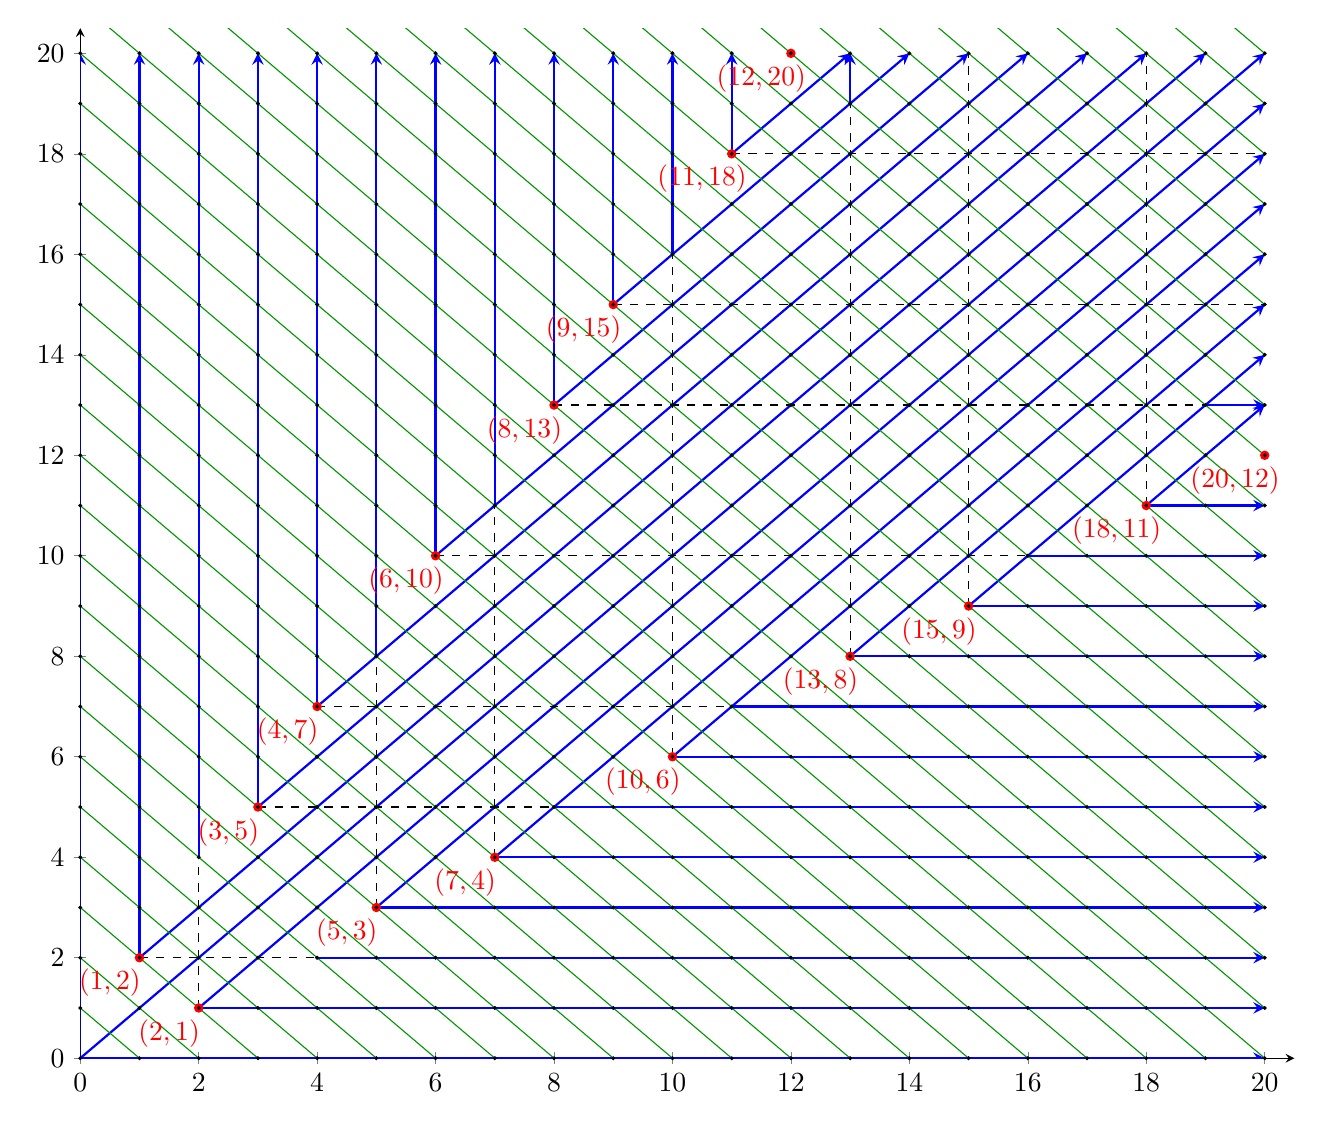
\begin{tikzpicture}
		\begin{axis}[
				xmin=0, xmax=20.5,
				ymin=0, ymax=20.5,
				axis lines = left,
			]
			\addplot[blue, thick, quiver={u=\thisrow{u},v=\thisrow{v}},-stealth] table {
				x y u v
				0 0 0 20
				0 0 20 0
				0 0 20 20
				2 1 18 0
				2 1 18 18
				2 4 0 16
				1 2 0 18
				1 2 18 18
				4 2 16 0
				3 5 0 15
				3 5 15 15
				8 5 12 0
				5 3 15 0
				5 3 15 15
				5 8 0 12
				4 7 0 13
				4 7 13 13
				11 7 9 0
				7 4 13 0
				7 4 13 13
				7 11 0 9
				6 10 0 10
				6 10 10 10
				16 10 4 0
				10 6 10 0
				10 6 10 10
				10 16 0 4
				8 13 0 7
				8 13 7 7
				19 13 1 0
				13 8 7 0
				13 8 7 7
				13 19 0 1
				9 15 0 5
				9 15 5 5
				15 9 5 0
				15 9 5 5
				11 18 0 2
				11 18 2 2
				18 11 2 0
				18 11 2 2
			};
		\addplot[black, dashed, quiver={u=\thisrow{u},v=\thisrow{v}}] table {
				x y u v
				2 1 0 3
				1 2 3 0
				3 5 5 0
				5 3 0 5
				7 4 0 7
				4 7 7 0
				6 10 10 0
				10 6 0 10
				8 13 11 0
				13 8 0 11
				9 15 11 0
				15 9 0 11
				11 18 9 0
				18 11 0 9
			};
		\addplot[fgreen, domain=0:20] {-x+1};
		\addplot[fgreen, domain=0:20] {-x+2};
		\addplot[fgreen, domain=0:20] {-x+3};
		\addplot[fgreen, domain=0:20] {-x+4};
		\addplot[fgreen, domain=0:20] {-x+5};
		\addplot[fgreen, domain=0:20] {-x+6};
		\addplot[fgreen, domain=0:20] {-x+7};
		\addplot[fgreen, domain=0:20] {-x+8};
		\addplot[fgreen, domain=0:20] {-x+9};
		\addplot[fgreen, domain=0:20] {-x+10};
		\addplot[fgreen, domain=0:20] {-x+11};
		\addplot[fgreen, domain=0:20] {-x+12};
		\addplot[fgreen, domain=0:20] {-x+13};
		\addplot[fgreen, domain=0:20] {-x+14};
		\addplot[fgreen, domain=0:20] {-x+15};
		\addplot[fgreen, domain=0:20] {-x+16};
		\addplot[fgreen, domain=0:20] {-x+17};
		\addplot[fgreen, domain=0:20] {-x+18};
		\addplot[fgreen, domain=0:20] {-x+19};
		\addplot[fgreen, domain=0:20] {-x+20};
		\addplot[fgreen, domain=0:20] {-x+21};
		\addplot[fgreen, domain=0:20] {-x+22};
		\addplot[fgreen, domain=0:20] {-x+23};
		\addplot[fgreen, domain=0:20] {-x+24};
		\addplot[fgreen, domain=0:20] {-x+25};
		\addplot[fgreen, domain=0:20] {-x+26};
		\addplot[fgreen, domain=0:20] {-x+27};
		\addplot[fgreen, domain=0:20] {-x+28};
		\addplot[fgreen, domain=0:20] {-x+29};
		\addplot[fgreen, domain=0:20] {-x+30};
		\addplot[fgreen, domain=0:20] {-x+31};
		\addplot[fgreen, domain=0:20] {-x+32};
		\addplot[fgreen, domain=0:20] {-x+33};
		\addplot[fgreen, domain=0:20] {-x+34};
		\addplot[fgreen, domain=0:20] {-x+35};
		\addplot[fgreen, domain=0:20] {-x+36};
		\addplot[fgreen, domain=0:20] {-x+37};
		\addplot[fgreen, domain=0:20] {-x+38};
		\addplot[fgreen, domain=0:20] {-x+39};
		\addplot[fgreen, domain=0:20] {-x+40};
		\addplot[red, only marks, mark=*, mark size=1.5pt] coordinates {
				(2,1)(1,2)(3,5)(5,3)(4,7)(7,4)(6,10)(10,6)(8,13)(13,8)(9,15)(15,9)(11,18)(18,11)(12,20)(20,12)
			};
			\foreach \x in {0,...,20} {
				\foreach \y in {0,...,20} {
					\addplot[black, only marks, mark=*, mark size = 0.5] coordinates {(\x,\y)};
				};
			};
			\draw node[red] at (0.5,1.5) {$(1,2)$};
			\draw node[red] at (2.5,4.5) {$(3,5)$};
			\draw node[red] at (3.5,6.5) {$(4,7)$};
			\draw node[red] at (5.5,9.5) {$(6,10)$};
			\draw node[red] at (7.5,12.5) {$(8,13)$};
			\draw node[red] at (8.5,14.5) {$(9,15)$};
			\draw node[red] at (10.5,17.5) {$(11,18)$};
			\draw node[red] at (11.5,19.5) {$(12,20)$};

			\draw node[red] at (1.5,0.5) {$(2,1)$};
			\draw node[red] at (4.5,2.5) {$(5,3)$};
			\draw node[red] at (6.5,3.5) {$(7,4)$};
			\draw node[red] at (9.5,5.5) {$(10,6)$};
			\draw node[red] at (12.5,7.5) {$(13,8)$};
			\draw node[red] at (14.5,8.5) {$(15,9)$};
			\draw node[red] at (17.5,10.5) {$(18,11)$};
			\draw node[red] at (19.5,11.5) {$(20,12)$};
		\end{axis}
	\end{tikzpicture}
\end{center}
\end{document}
